\section{Results and discussion}\label{results.sec}

%\subsection{Comparison of SLAC E139 and E03-103 kinematics}\label{kinemcomp.ssec}

Before presenting the results, it is instructive to compare our kinematics to
the earlier SLAC experiments. This will help identify potential issues the
comparison of the results and examinations of the $Q^2$ dependence when
combining data from different experiments. Figure~\ref{slac_e0103_kinem_fig}
shows kinematics for our measurement and SLAC E139 and E140.

E03-103 took data on all targets at 40$^\circ$ and 50$^\circ$, and the cross
section ratios with respect to deuterium were extracted.  The EMC ratios are
extracted from the 40 degree angle (solid line in
Fig.~\ref{slac_e0103_kinem_fig}) where the data have better statistics and
more complete kinematic coverage. Data were also collected for a detailed $Q^2$
dependency study at 8 additional kinematic settings on C and $^2$H.

\begin{figure}[htbp]
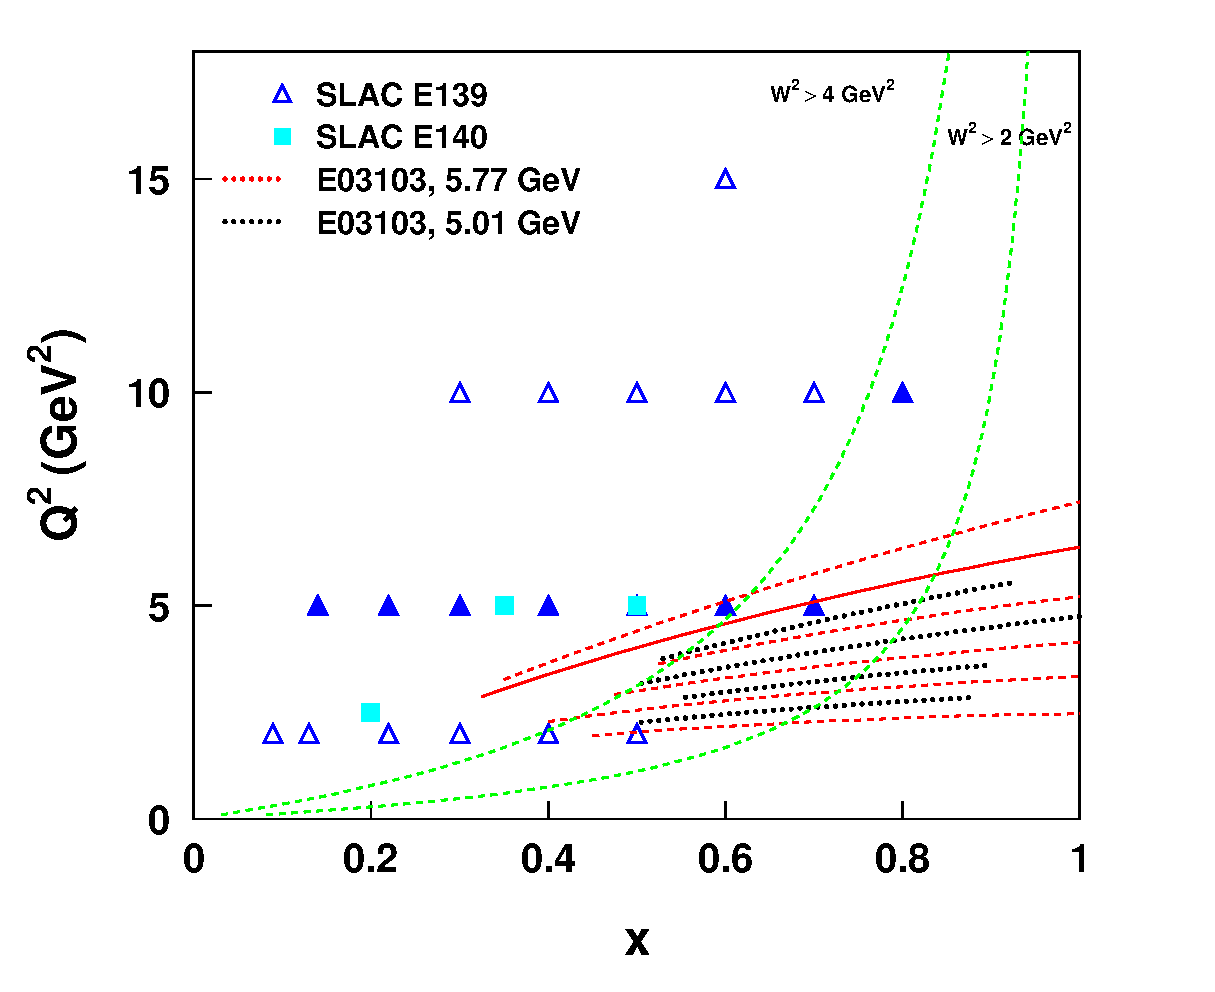
\includegraphics[width=.45\textwidth]{plots/slac_e03103_x_q2.eps}
\caption{(Color online) The E03-103 kinematics, indicated with dashed and
dotted lines, along with the SLAC experiments E139~\cite{slace139} (triangles)
and SLAC E140~\cite{slace140} (squares).  Kinematics are shown for the target
with maximum coverage (Fe for the SLAC measurements, C for E03-103). The solid
line and filled symbols represent the kinematics used in the main comparison
of the results. Contours of constant invariant mass squared are also shown in
the figure.
\label{slac_e0103_kinem_fig}}
\end{figure}

In the cross section ratio plots, representative world data is also displayed
with the corresponding nuclei where available. In the kinematics
comparison plot we chose to display kinematics of SLAC experiments because of
the overlap in kinematics with our experiment at high $x$. For comparison of
the EMC ratios we use the SLAC data at $Q^2=5$~GeV$^2$, except for the highest
$x$, where $Q^2=10$~GeV$^2$. For each $x$, $Q^2$ value, published SLAC E140
results are averaged over several $\epsilon$ points and we will come back to
this point latter in this section.

To be consistent, the presented SLAC data have updated Coulomb and isoscalar
corrections using the same prescriptions used for the analysis of E03-103
data. The updated data points and corrections factors are available in the
supplementary online material~\cite{online_material}.



%========================================================

\subsection{$Q^2$ dependence of the ratios}\label{q2depresult.ssec}

\begin{figure}[htbp]
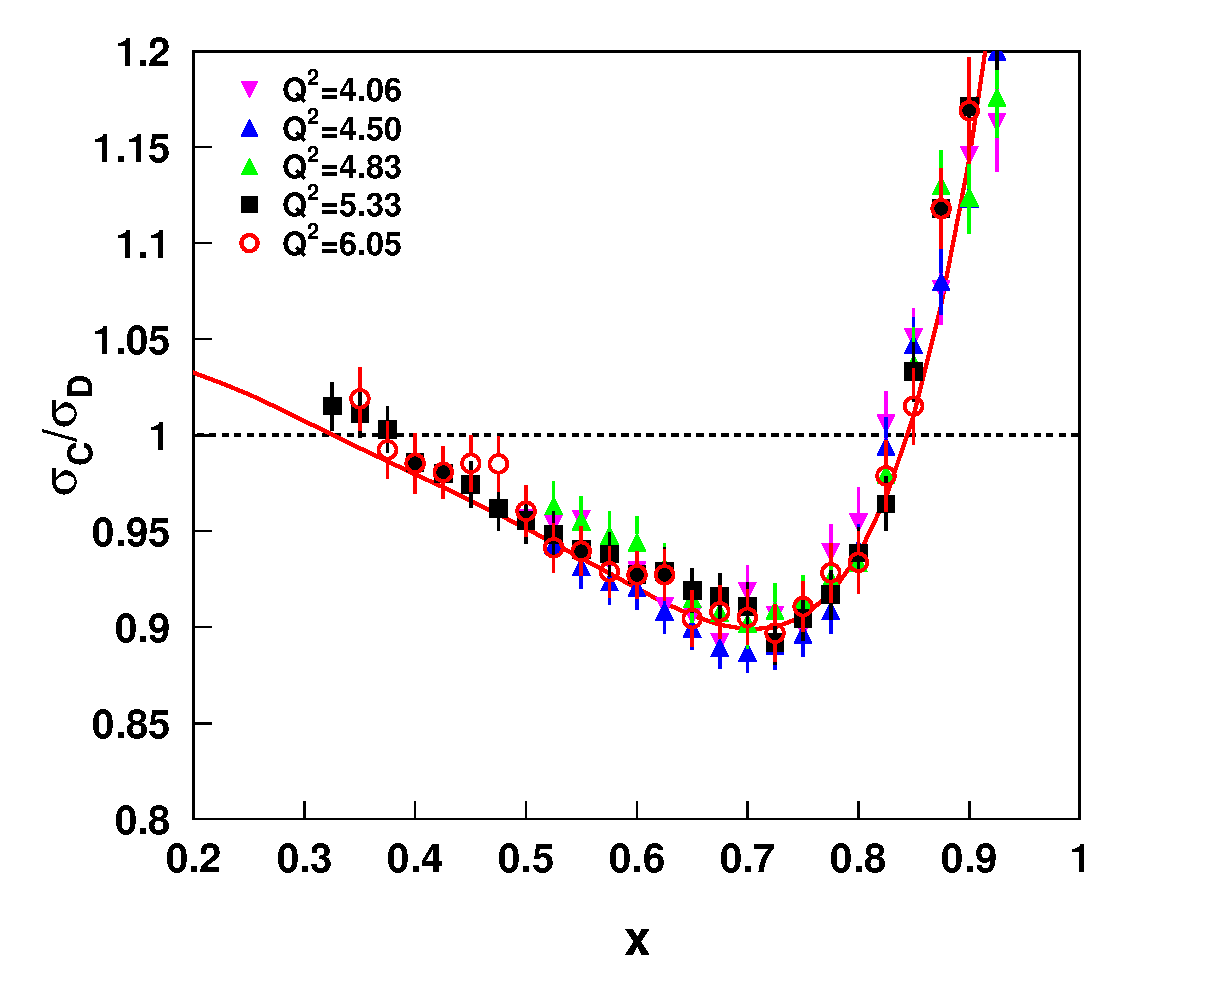
\includegraphics[width=.44\textwidth,height=55mm]{plots/e03103_C_hiq2_x_scaling.eps}
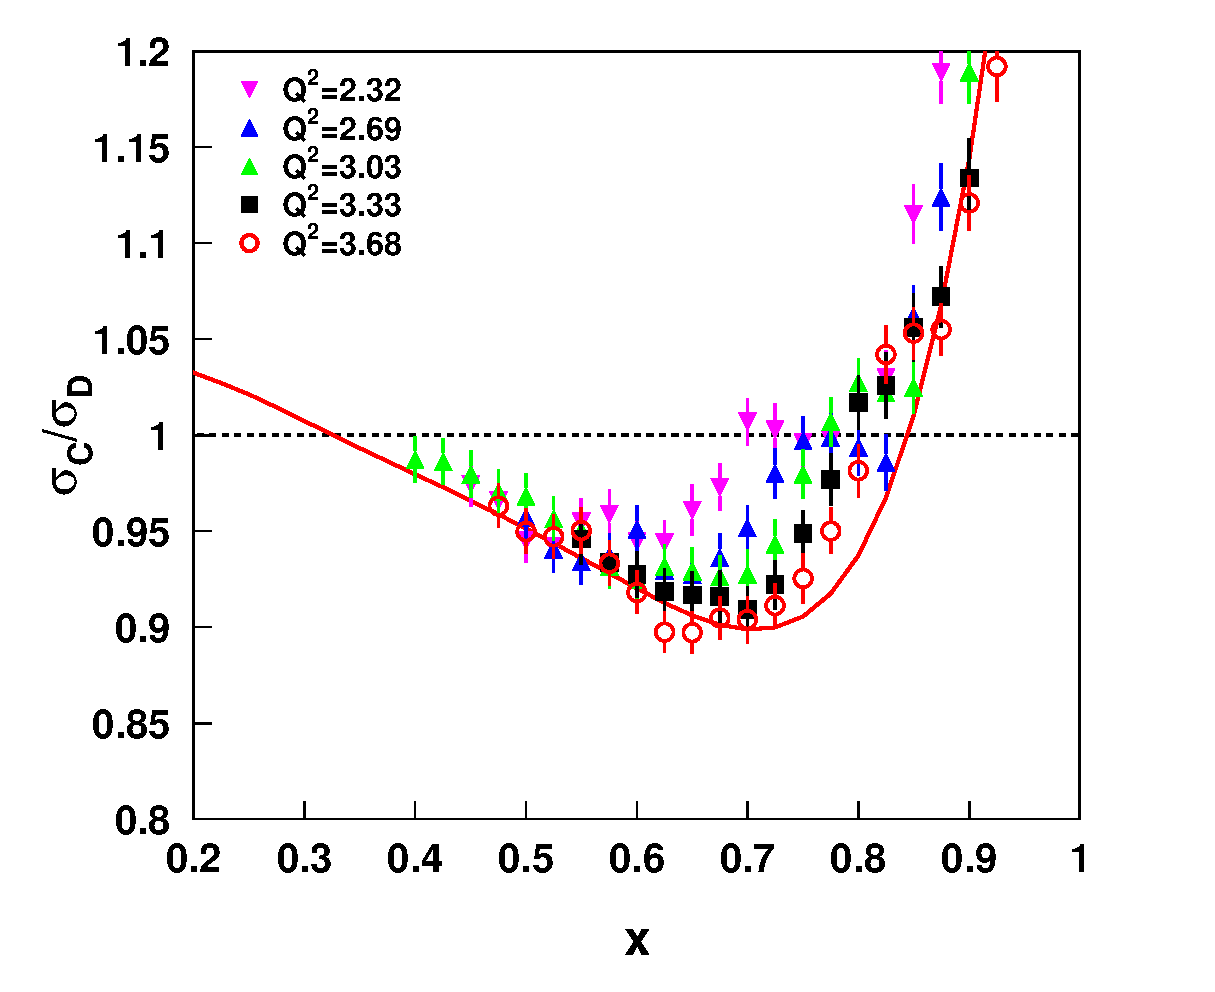
\includegraphics[width=.44\textwidth,height=55mm]{plots/e03103_C_loq2_x_scaling.eps}
\caption{Ratio of C and $^2$H cross sections for the five largest $Q^2$ (top
panel) and five lowest $Q^2$ (bottom panel) settings as a function of $x$.
Uncertainties are the combined statistical and point-to-point systematic. The
$Q^2$ values quoted are for $x=0.75$, and the data labeled $Q^2$=5.33
correspond to our primary results, taken at 40$^\circ$.
\label{emc_x_C_hiq2dep_fig}}
\end{figure} 

The scaling of the structure functions for nucleons is expected to hold 
in the conventional DIS region ($W^2>4$ and $Q^2>1$), where the
non-perturbative, resonance structure is no longer apparent and only
QCD evolution yields a $Q^2$ dependence. At smaller values
of $W^2$, corresponding to large $x$, additional scaling violations can
originate from resonance contributions. For E03-103, the data are in the
conventional DIS region up to $x \approx 0.6$.  There are indications
\cite{Arrington:2003nt} that the nuclear structure functions in the resonance
region, down to very low $W^2$ values ($W^2 > 1.5$~GeV$^2$ for
$Q^2>3$~GeV$^2$), shows the same global behavior as in the DIS region. 
Therefore, we took data at large $x$ extending below $W^2=4$~GeV$^2$, and made
detailed measurements of the $Q^2$ dependence of the ratios to ensure that
there was no indication of any systematic deviation from the DIS limit.

The EMC ratios for carbon at several $Q^2$ values are compared in
Fig.~\ref{emc_x_C_hiq2dep_fig}.  The top panel shows the EMC ratios for the
five highest $Q^2$ settings from our experiment, along with our new
parametrization for the EMC effect (see section~\ref{emcparam.ssec}).  The
data do not show any systematic $Q^2$ dependence, and the scatter at the
largest $x$ values is consistent with the uncertainties in the individual
measurements.  This suggests that any $Q^2$ dependence in the structure
function is either small or cancels in the target ratios.  The bottom figure
shows the low $Q^2$ measurements, where there is a clear difference in the
$Q^2$ dependence of carbon and deuterium below $Q^2 \approx 3$~GeV$^2$ and
$x>0.6$, corresponding to $W^2$ values below 2--3~GeV$^2$, where one expects
large resonance contributions.


\begin{figure}[htbp]
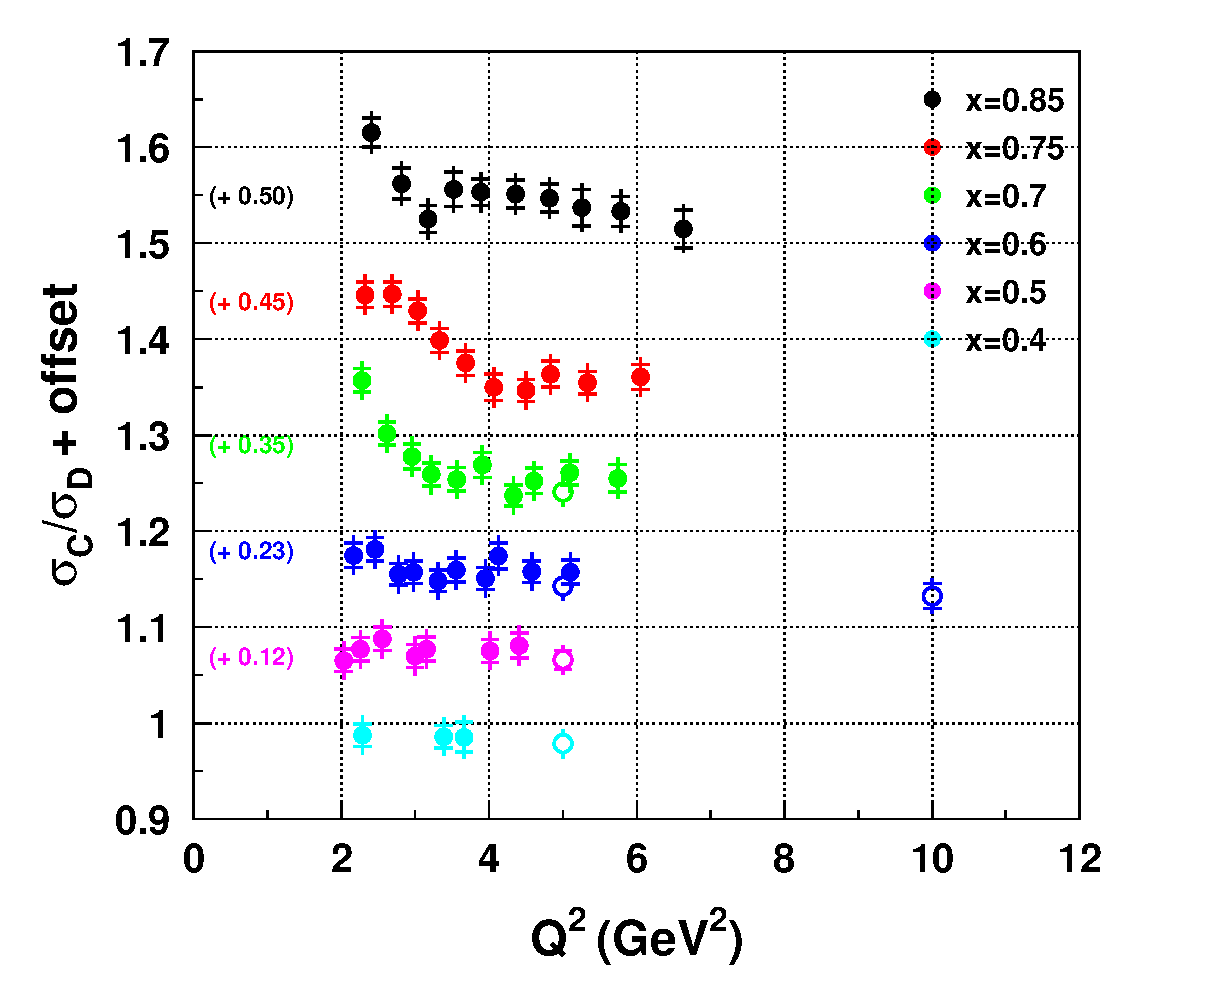
\includegraphics[width=.44\textwidth,height=55mm]{plots/compare_slac_c_q2dep.eps} \\
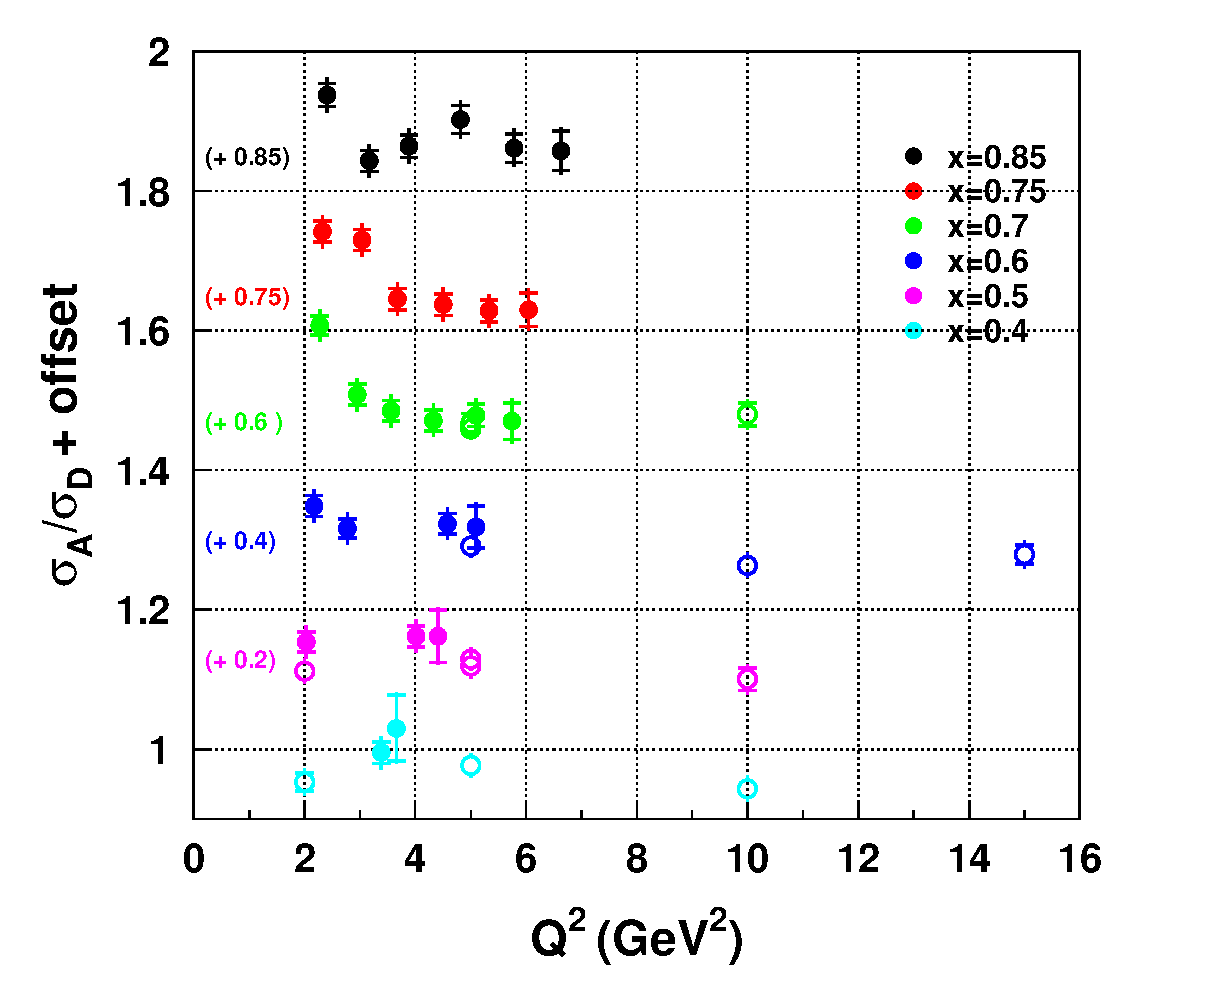
\includegraphics[width=.44\textwidth,height=55mm]{plots/compare_slac_cu_q2dep.eps}
\caption{EMC ratios for the C data (top) and the Cu and Fe data (bottom) as a
function of $Q^2$ at fixed $x$ values as indicated in legend. For clarity, an
additive offset is applied along the y axis. Open symbols are from updated
SLAC E139~\cite{slace139} results while the closed symbols are E03-103 values.
Inner error bars shows the combined statistical and point-to-point systematic
while the outer error bars represents the total uncertainty including the
normalization uncertainties.
\label{emc_q2_c_fixed_x_fig}}
\end{figure}



Figure~\ref{emc_q2_c_fixed_x_fig} shows the $Q^2$ dependence of the structure
functions for C (top) and Cu or Fe (bottom) at several $x$ values, to allow
for a more careful examination of the $Q^2$ dependence as a function of $x$. 
The carbon data have additional $Q^2$ values for E03-103, due to the data
taken using a lower beam energy, while the Cu data have more high-$Q^2$
data from the SLAC measurements. There is a fair agreement with the SLAC data
over the kinematic regions where data are available, and clear deviations from
a constant ratio are visible below $Q^2=4$~GeV$^2$ and large $x$ values.

%\begin{figure}[htbp]
%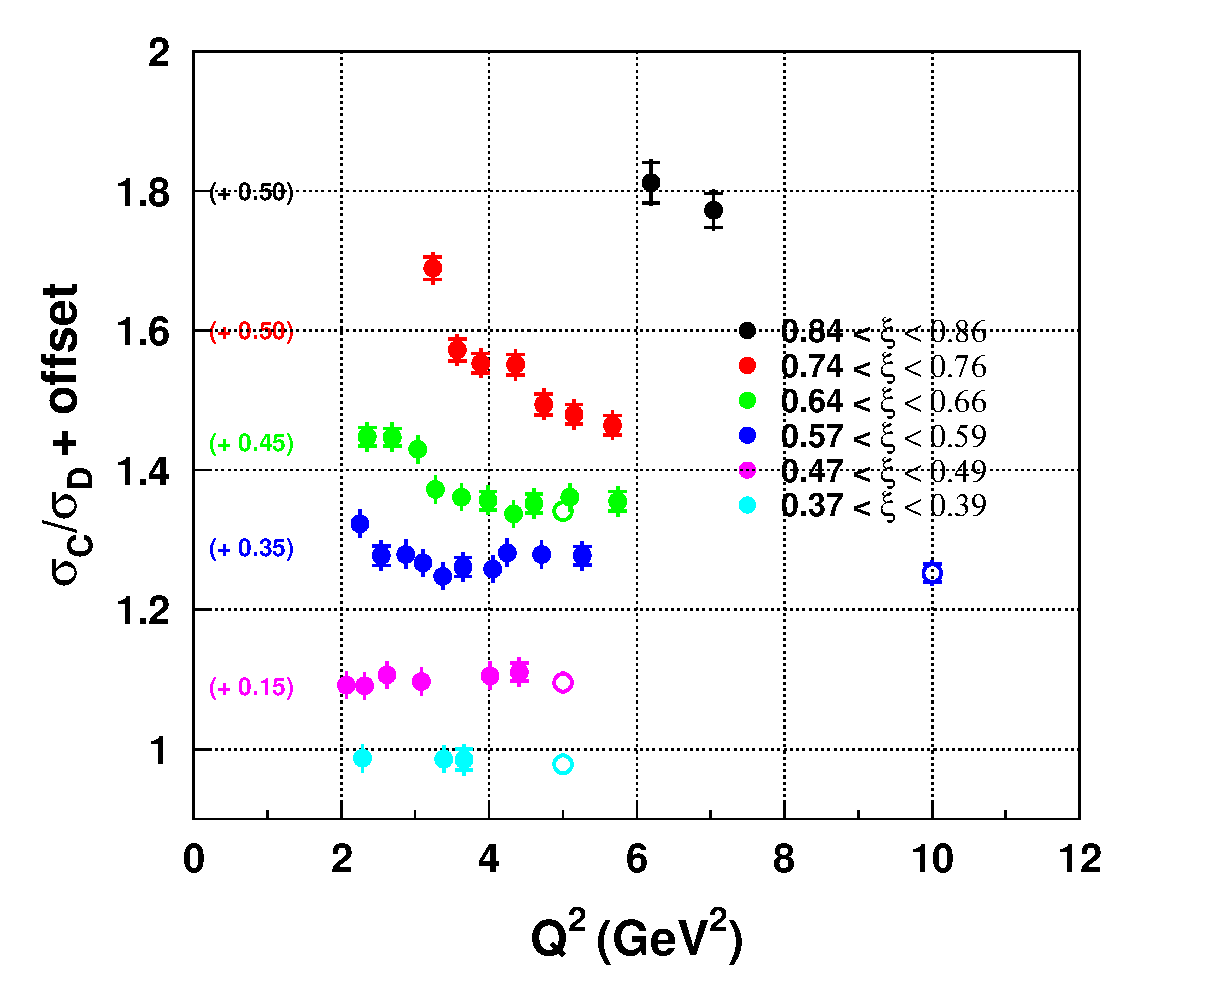
\includegraphics[width=.44\textwidth,height=55mm]{plots/compare_slac_c_q2dep_fixedxi.eps}
%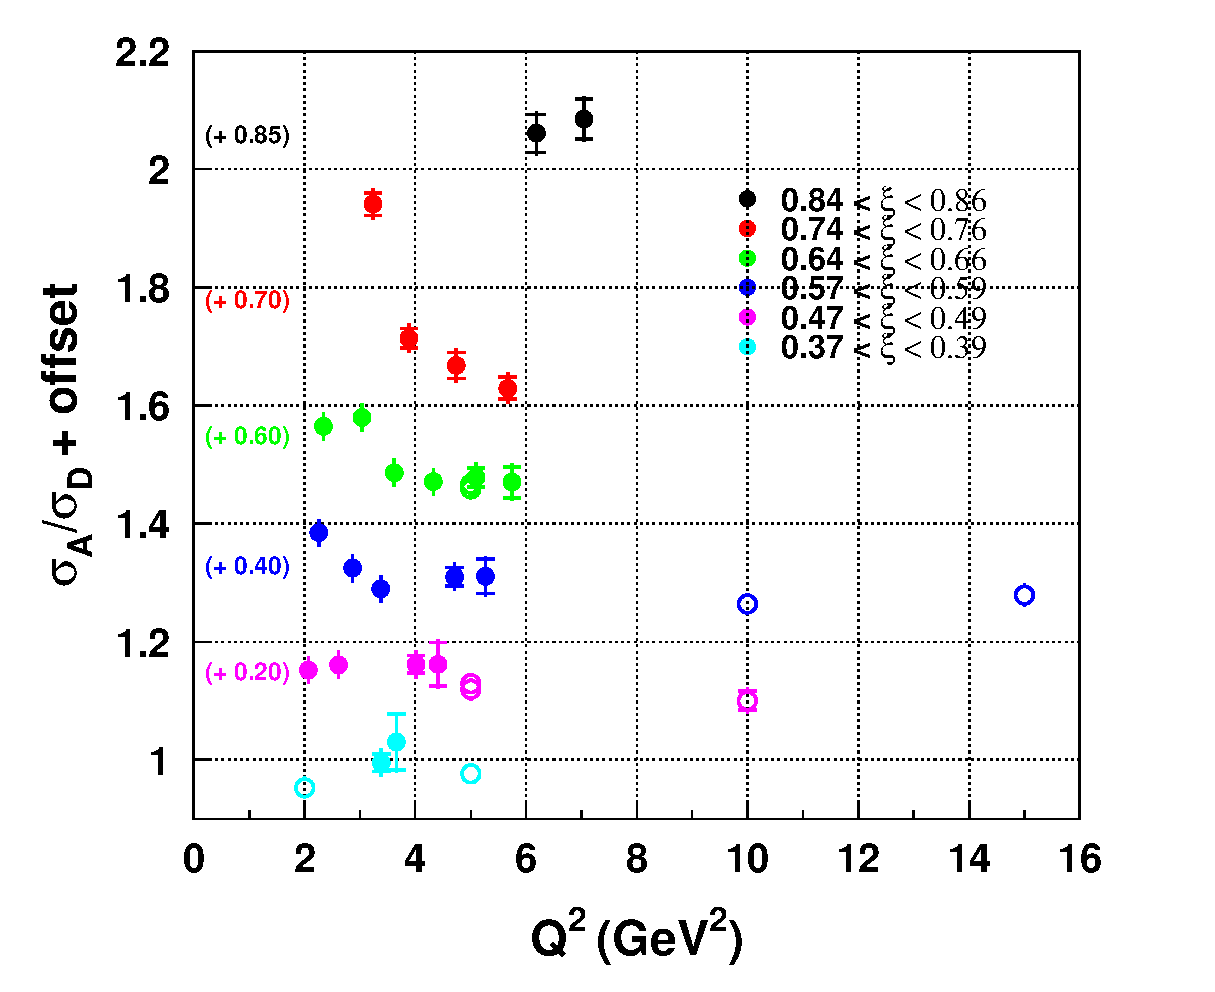
\includegraphics[width=.44\textwidth,height=55mm]{plots/compare_slac_cu_q2dep_fixedxi.eps}
%caption{EMC ratios for the C (top) and Cu (bottom) targets as a function of
%$Q^2$ at different $\xi$ intervals as indicated in legend. For clarity, an
%arbitrary additive offset (as shown in the figure) is applied along the y
%axis. Open symbols are from updated SLAC E139 results while the closed symbols
%are E03-103 values. Inner error bars shows the combined statistical and
%point-to-point systematic while the outer error bars represents the total
%uncertainty including the normalization uncertainties.
%\label{emc_q2_c_fixed_xi_fig}}
%\end{figure}

%For the individual structure functions, the largest $Q^2$ dependence in this
%region is associated with the so-called ``target-mass
%corrections''~\cite{Schienbein_tarmass_rev}. 

%In the DIS region, we see scaling not only in variable $x$, but also in the
%Nachtmann variable $\xi$. For very large $Q^2$, $\xi \rightarrow x$, and in
%the DIS limit $\xi$ is related to the quark momentum distribution, as is the
%case for $x$. However, scaling violations at finite $Q^2$ are smaller when
%we examine the data in terms of $\xi$ rather than $x$, because using this
%variable partially accounts for target mass effects.
%Fig~\ref{emc_q2_c_fixed_xi_fig} shows the EMC ratios for the C target as a
%function of $Q^2$ at different $\xi$ intervals as indicated in legend.

%\textit{JRA: Removed plots of $Q^2$ dependence at fixed $\xi$.  For structure
%functions (rather than ratios), it should reduce scaling violations.  For
%the ratios, the part we're showing mainly just shifts strength in $x$ or $\xi$.
%So it makes a big difference in showing the $x$ vs. $\xi$ dependence, but has
%less impact on the $Q^2$ dependence.  If we want to put it back we can, but
%it will need a better introduction/explanation unless we just want to say
%that we show it for completeness, and refer back to TMC discussion in previous
%section. I'm also not a big fan of taking an interval in $\xi$, so if we decide
%to show it, we should probably interpolate to fixed $\xi$ values, and modify
%the values so that they match the $x$ values of the high $Q^2$ SLAC data
%(e.g. so that we can include SLAC data, and also not have the high-$\xi$ point
%such that most of the data is off scale}.


%========================================================
\subsection{$x$ dependence of the ratios}\label{xdepresult.ssec}


\textit{Need to summarized differences from PRL values (e.g. isoscalar
correction) and errors (added CC error).}

\begin{figure}[htbp]
\begin{center}
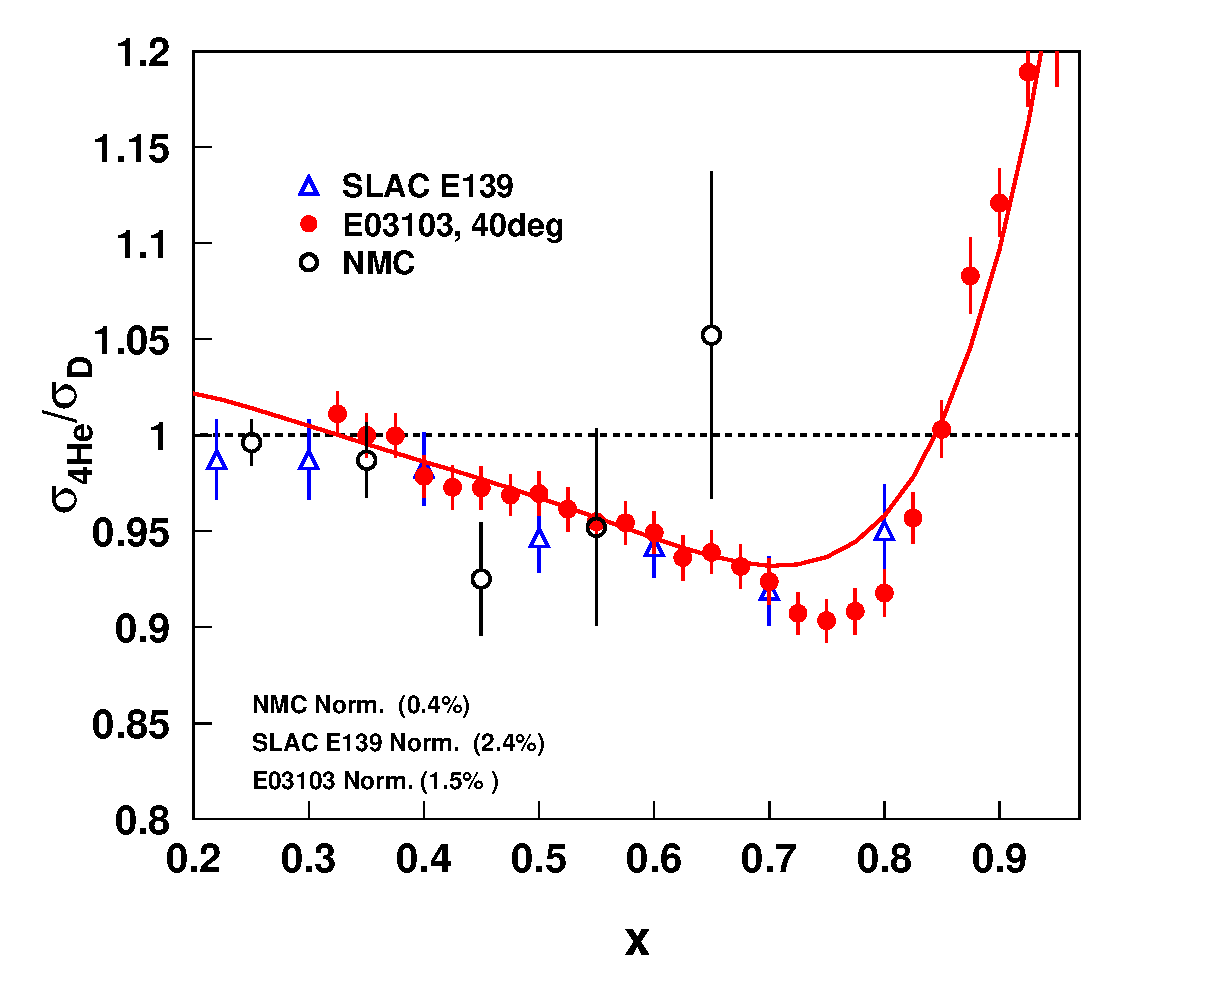
\includegraphics[width=.44\textwidth,height=55mm]{plots/slacWithallcorr_e03103_40deg_emc_x_he4.eps}
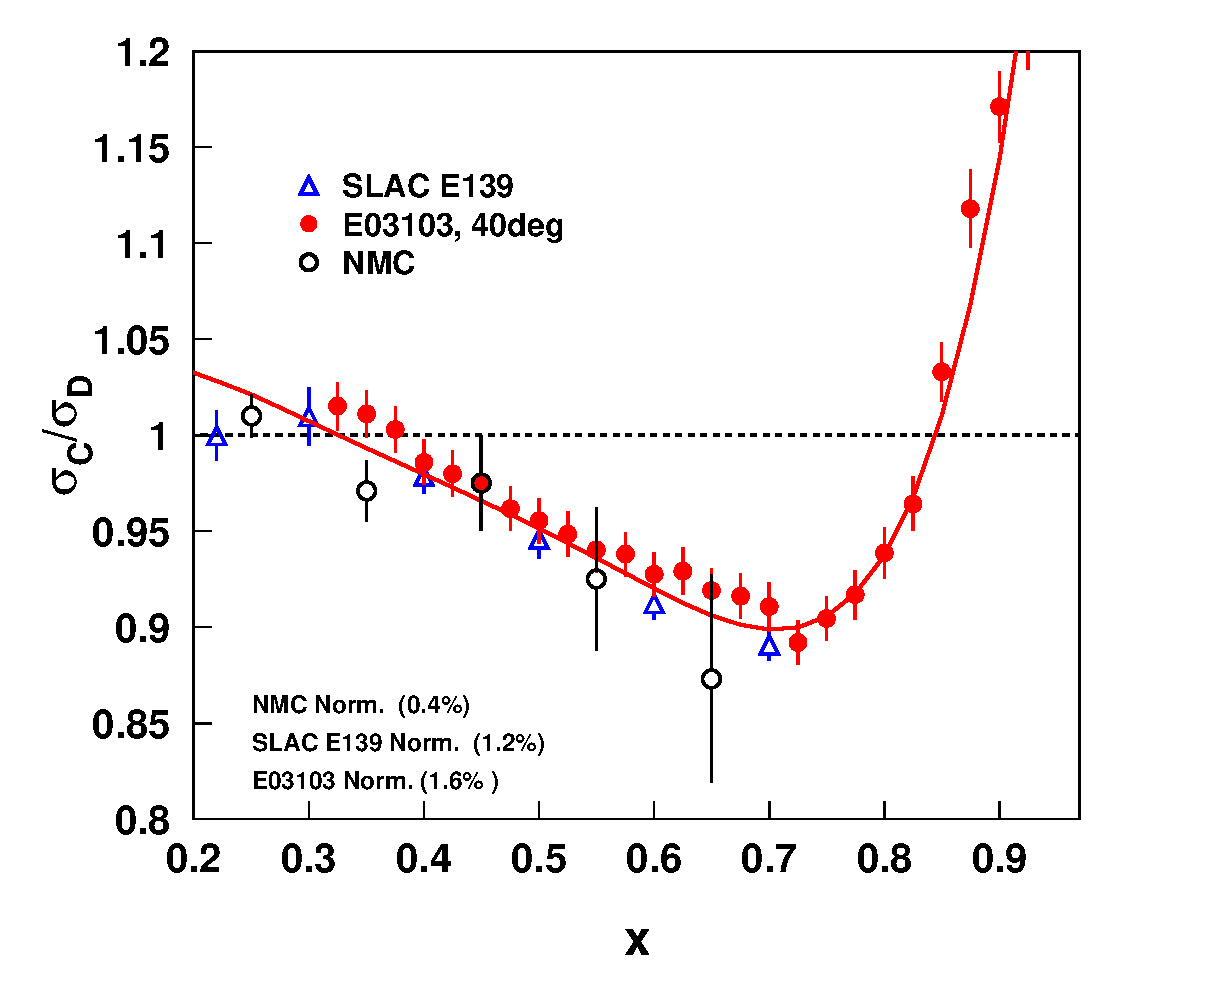
\includegraphics[width=.44\textwidth,height=55mm]{plots/slacWithallcorr_e03103_40deg_emc_x_c12.eps}
\caption{EMC ratios for $^4$He and $^{12}$C as a function of $x$ for the 40
degree data. Uncertainties are the combined statistical and point-to-point
systematic. Normalization uncertainties are shown in the parenthesis. Also
shown are the updated SLAC E139~\cite{slace139} and NMC data
\cite{Arneodo:1995cs, Amaudruz:1995tq}. The solid curves show our A dependent
parametrization for
the EMC effect.
\textit{NMC data is as-published, not updated.  Is the fit OURS or the SLAC
fit?  Mention differences in error bar in text?}
\label{emc_x_40deg_he4_fig}}
\end{center}
\end{figure}


We now examine the $x$ dependence of the EMC ratios for all of the targets
from E03-103 and SLAC, including Coulomb corrections and our updated isoscalar
corrections. We first discuss the cross section ratios for C and $^4$He, as
these ratios have no isoscalar correction, and the Coulomb distortion effects
are small ($<$1\%) for these nuclei. Figure~\ref{emc_x_40deg_he4_fig} shows
the cross section ratios for $^4$He and $^{12}$C, along with the updated SLAC
E139 data and the NMC data~\cite{Amaudruz:1995tq,Arneodo:1995cs}. There is a
good agreement between the data sets, but the E03-103 result is of high
precision at large $x$, although it is at a lower $W^2$ than previous
measurements.



\begin{figure}[htbp]
\begin{center}
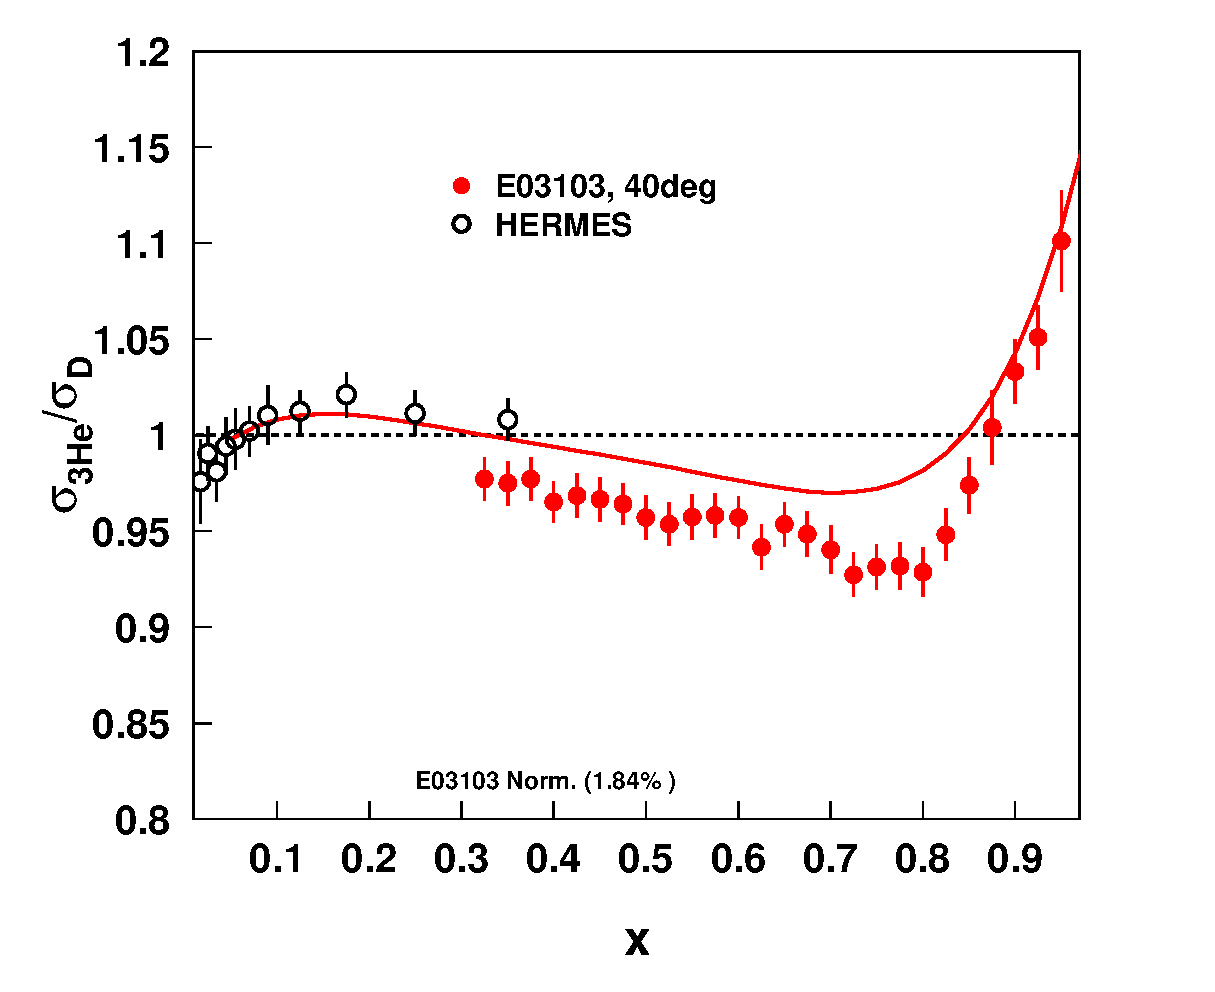
\includegraphics[width=.44\textwidth,height=55mm]{plots/slacWithallcorr_e03103_40deg_emc_x_he3.eps}
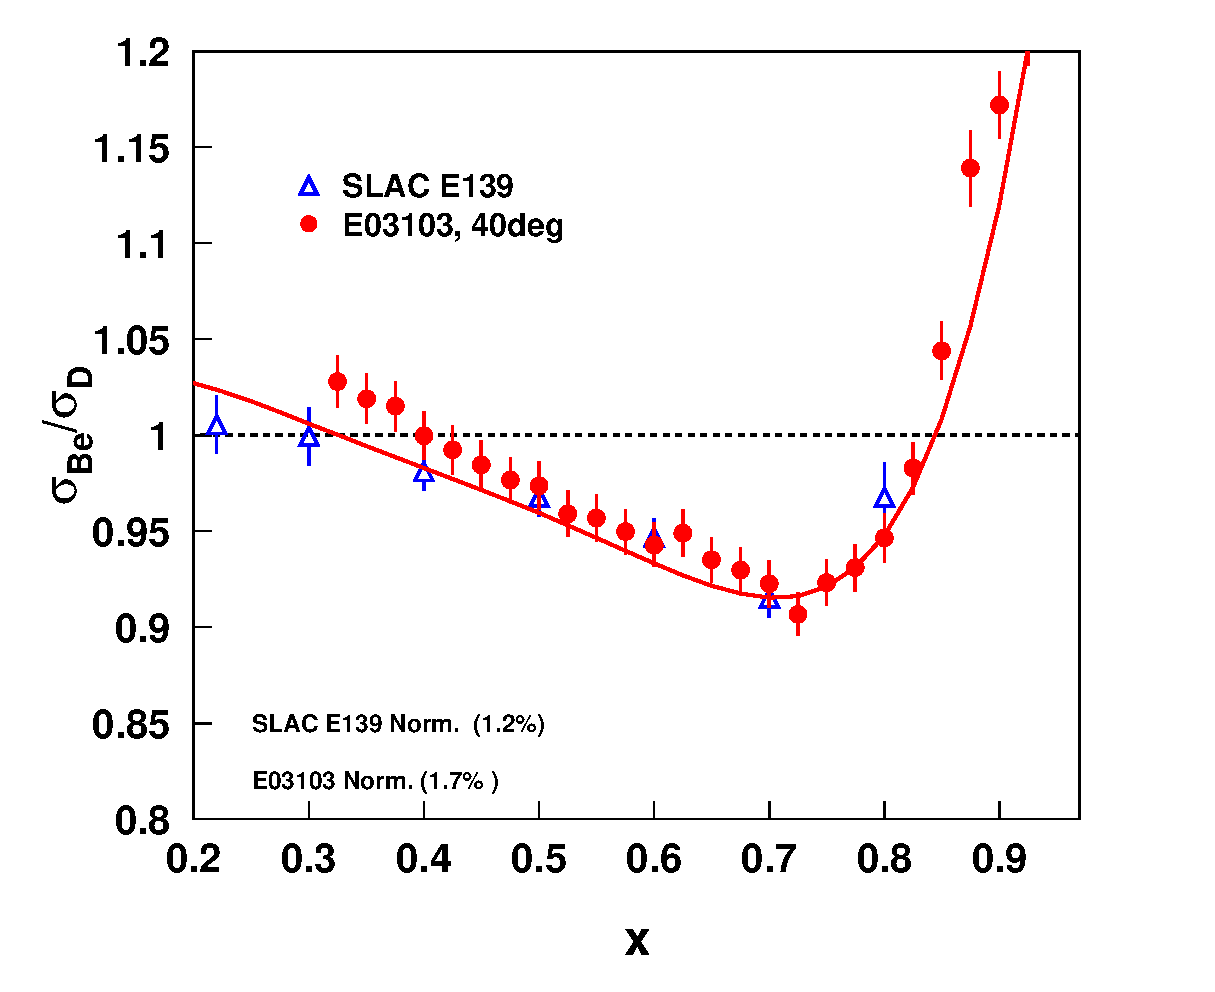
\includegraphics[width=.44\textwidth,height=55mm]{plots/slacWithallcorr_e03103_40deg_emc_x_be.eps}
\caption{Isoscalar EMC ratios for $^3$He and $^9$Be for the 40 degree data.
Uncertainties are the combined statistical and point-to-point systematic and
normalization uncertainties are shown in the parenthesis. Also shown are the
HERMES data~\cite{hermes_ackerstaff,hermes_correction_airapetian} (updated to
include our modified isoscalar correction). The solid curve shows an A
dependent parametrization for the EMC effect in $^3$He.
\label{emc_x_40deg_he3_fig}}
\end{center}
\end{figure}


Figure~\ref{emc_x_40deg_he3_fig} shows the cross section ratios for $^3$He
and $^9$Be.  Both of these nuclei are light enough that the Coulomb corrections
are small, but required a proton (neutron) excess correction to obtain the
isoscalar EMC ratios (see section~\ref{iso.ssec}). The magnitude of this
correction is significant for $^3$He, ranging from about $5\%$ to $15\%$ for
our kinematics.  For $^9$Be, the correction is of the opposite sign and
roughly a factor of three smaller.  The $^3$He EMC ratios exhibit the general
shape observed for the cross section ratios for heavy nuclei.

%Fig~\ref{emc_x_40deg_he3_fig} shows the isoscalar
%corrected along with the updated HERMES results.  It should be noted that the
%published HERMES results~\cite{hermes_ackerstaff,hermes_correction_airapetian}
%applied a proton excess correction that used the NMC parameterization for
%$F_2^n/F_2^p$, while our results are derived using the prescription discussed
%in section~\ref{iso.ssec}. To be consistent, HERMES data are reanalyzed to
%include the isoscalar corrections used in this analysis and are shown in Fig
%~\ref{emc_x_40deg_he3_fig}.

One can avoid the uncertainty associated with the isoscalar correction, and
thus better evaluate models of the EMC effect, by taking the ratio of $^3$He
to ($^2$H+$^1$H) which allows comparisons to calculations that are independent
of the neutron structure function.  These ratios are extracted for our 40
degree setting and shown in Figure~\ref{emc_x_40deg_he3_fig} (squares).
\textit{WRONG FIGURE!} 
The isoscalar-corrected $^3$He/$^2$H ratio and the $^3$He/($^2$H+$^1$H)
results are in good agreement below $x \approx 0.65$, but the resonance
structure at large $x$ in the proton is not washed out, and so the extended
scaling observed in nuclei~\cite{Arrington:2003nt} is not as effective,
limiting the useful range for this ratio to $x \ltorder 0.65$.



\begin{figure}[htbp]
\begin{center}
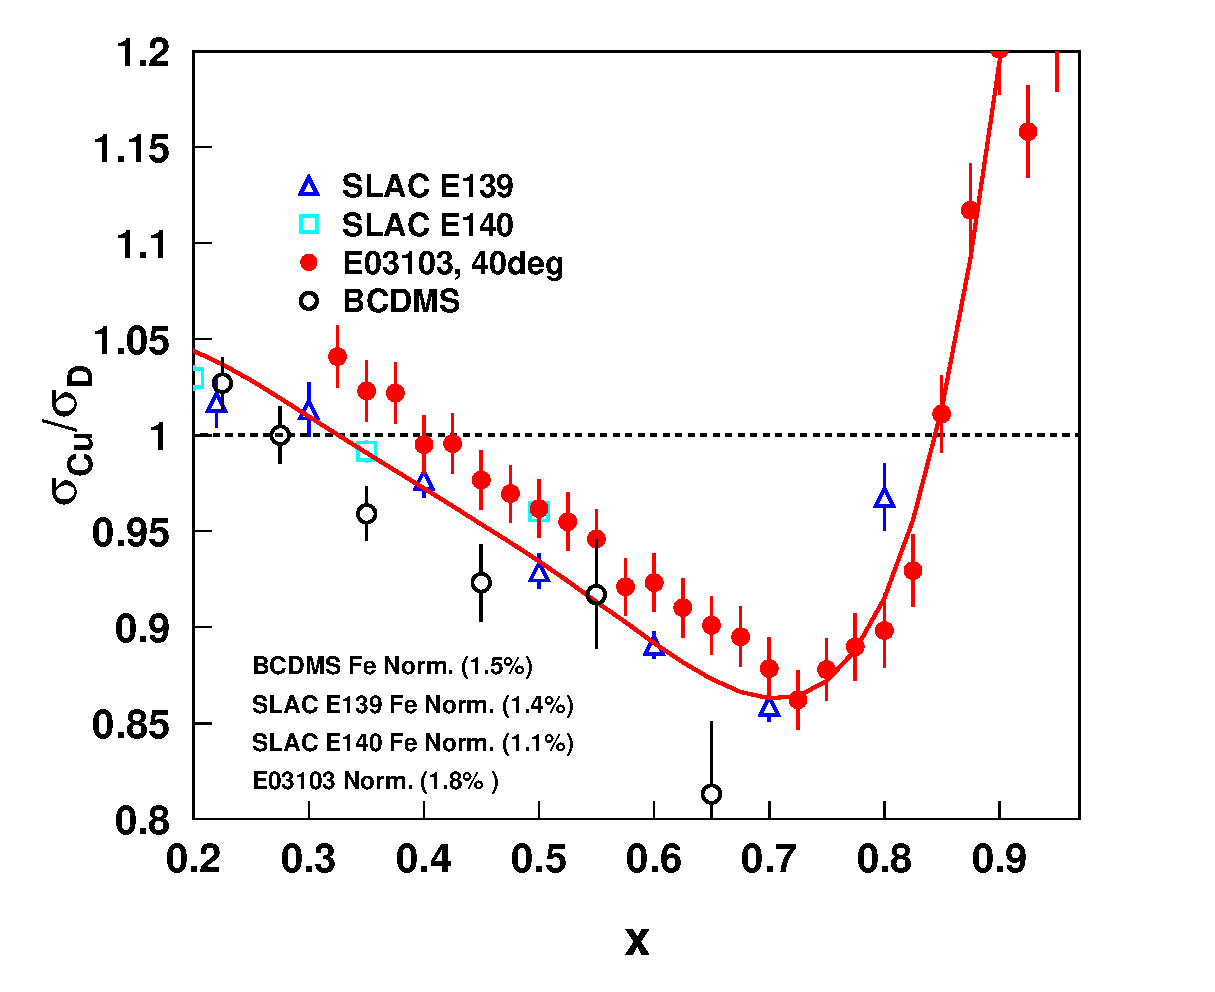
\includegraphics[width=.44\textwidth,height=55mm]{plots/slacWithallcorr_e03103_40deg_emc_x_cu_slace140loeps.eps}
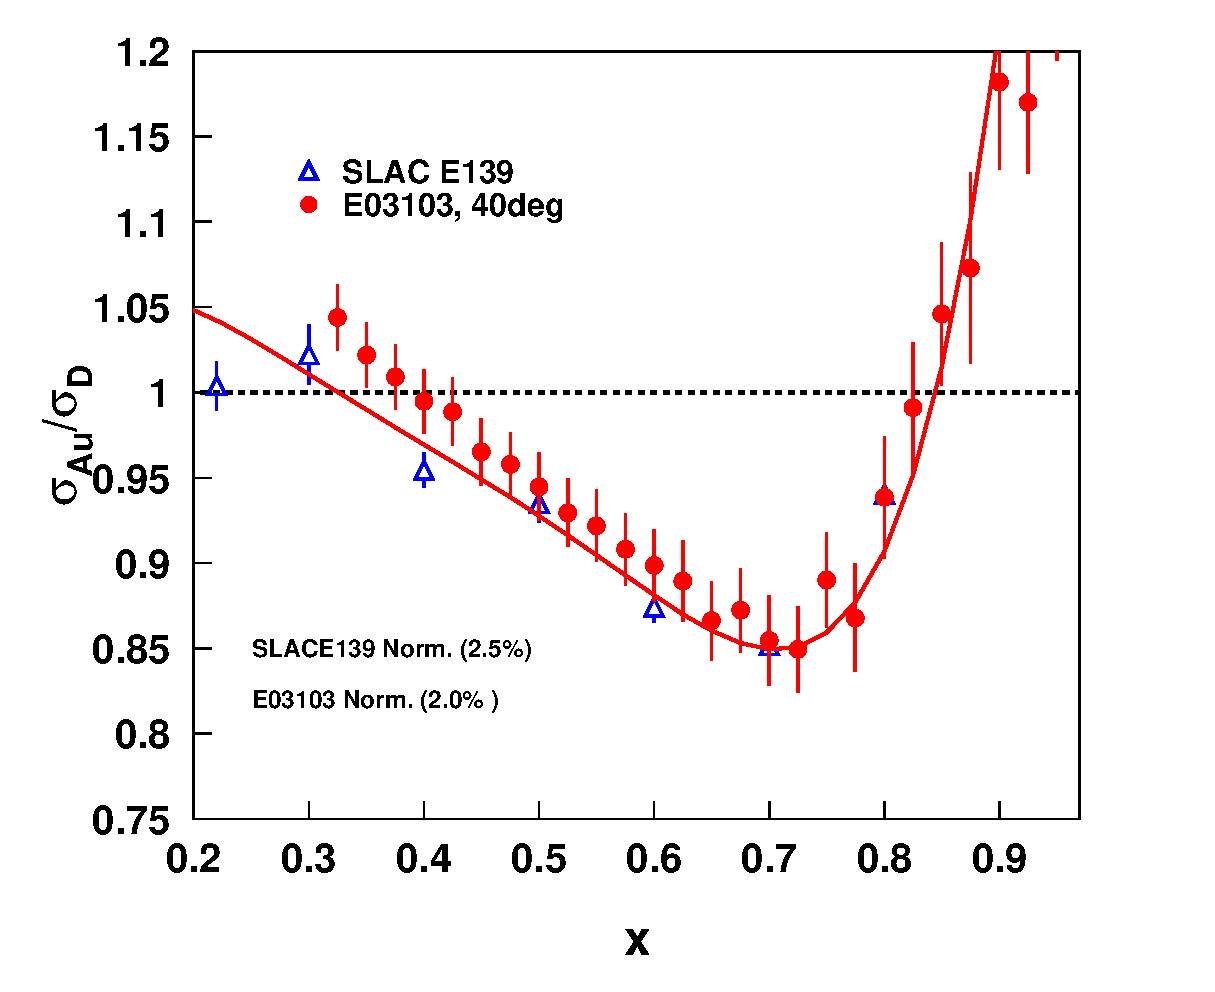
\includegraphics[width=.44\textwidth,height=55mm]{plots/slacWithallcorr_e03103_40deg_emc_x_au.eps}
\caption{EMC ratios for Fe and Cu (top) and for Au (bottom) as a function of
$x$ for the 40 degree data. Uncertainties are the combined statistical and
point-to-point systematic. Normalization uncertainties are shown in the
parenthesis. The SLAC E139 and E140 data include updated Coulomb and isoscalar
corrections. BCDMS~\cite{Benvenuti:1987az} Fe data are shown as published.
\label{emc_x_40deg_cu_fig}}
\end{center}
\end{figure}

Next, we show the ratios for heavy nuclei in Fig.~\ref{emc_x_40deg_cu_fig}.
Several corrections to the data on heavy nuclei are larger or more uncertain
than for light nuclei. At low $x$, the radiative corrections and charge
symmetric background (see section~\ref{csbg.sssec}) are quite large. At high
$x$, Coulomb distortion becomes large for high-Z targets; the correction for
Au ranges from 3\% at low $x$ to 12\% at high $x$ values for the 40$^\circ$
data.



\begin{figure}[htbp]
\begin{center}
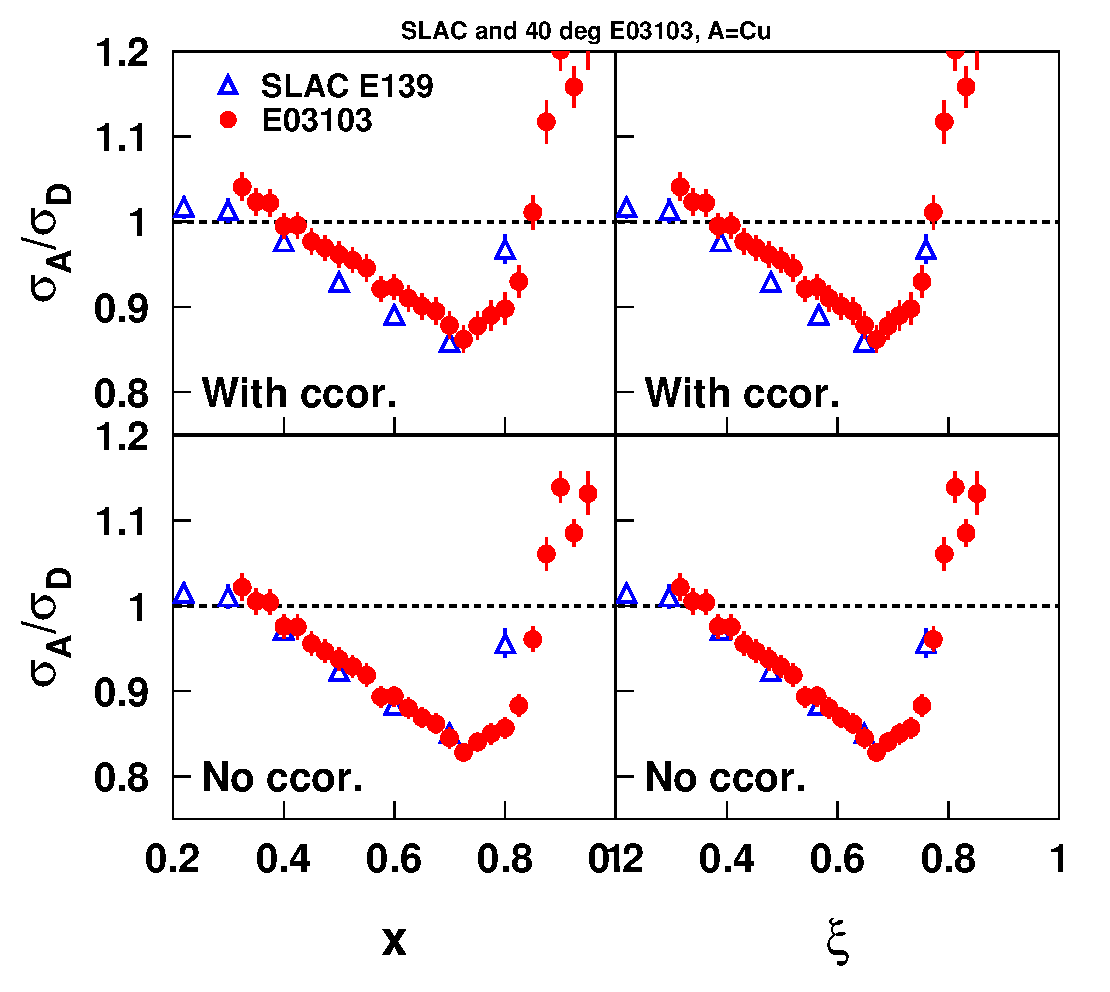
\includegraphics[width=.46\textwidth]{plots/e03103_slac_cu_2by2zone.eps}
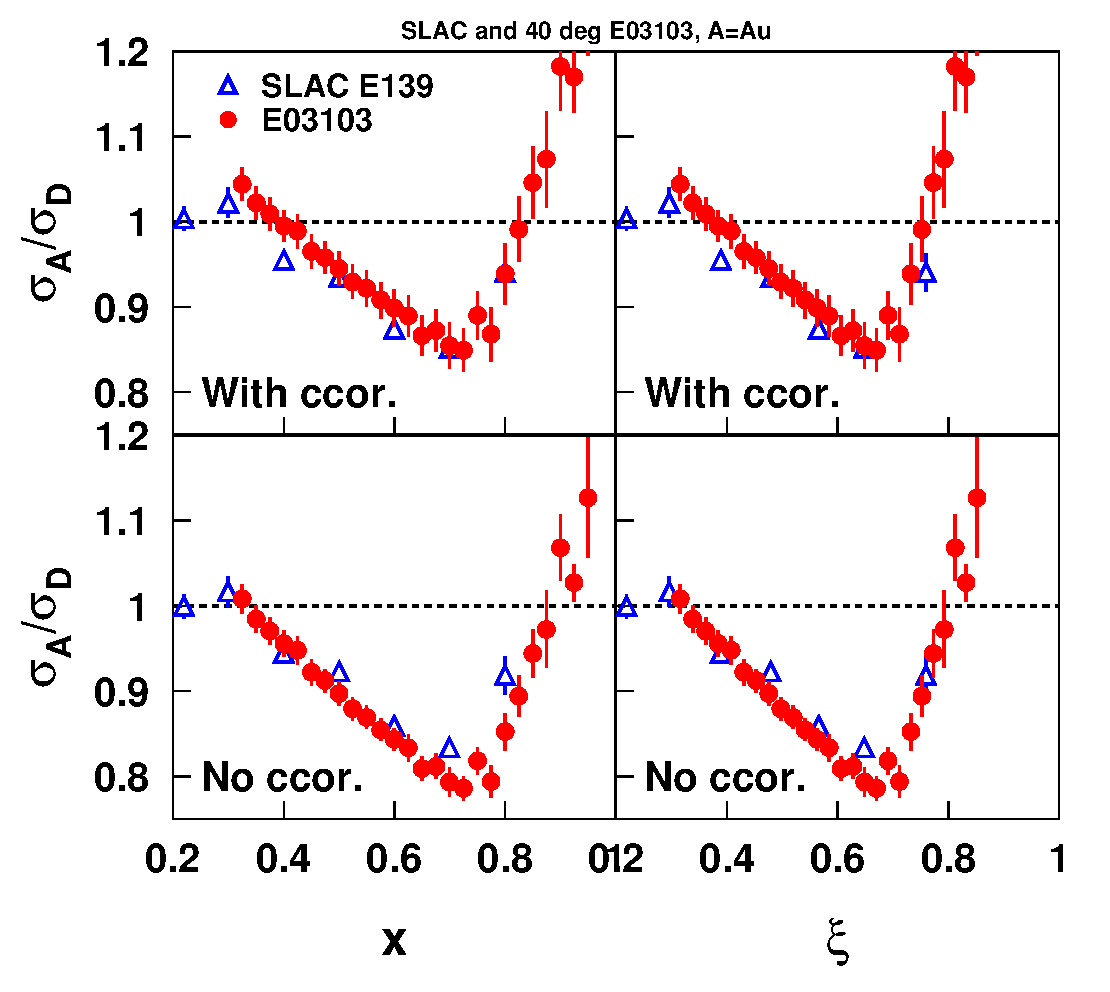
\includegraphics[width=.46\textwidth]{plots/e03103_slac_au_2by2zone.eps}
\caption{EMC ratios for our Cu (top) and Au (bottom) data compared to the
SLAC Fe and Au data, respectively, shown using four different sets of
corrections.  The panels on the left (right) side show the ratio vs $x$
($\xi$), while the panels on the top (bottom) show the ratios with (without)
Coulomb corrections applied. For each target, the top-right figure is the
version where one expects the best agreement between different measurements,
assuming that the Coulomb and target mass corrections account for any $\theta$
and $Q^2$ dependence in the cross section ratios.  For all nuclei, high-$x$
SLAC and JLab results are in good agreement, after taking into account the 
scale uncertainties in the measurements.
\label{emc_slac_2by2zone_cu_fig}}
\end{center}
\end{figure}

Taking normalization uncertainties into account, our large-$x$ results are in
generally good agreement with the SLAC data, although the SLAC ratios at
$x=0.8$ are always higher than our results.  This is because the $x=0.8$
points for SLAC are taken at higher $Q^2$ values ($Q^2=10$~GeV$^2$), leading
to a noticeable difference between the target mass corrections needed for the
two experiments. Figure~\ref{emc_slac_2by2zone_cu_fig} shows the points
plotted as a function of $x$ (left panels) and $\xi$ (right panels), where
plotting the ratio vs. $\xi$ provides the dominant part of the target mass
correction. While all of the points shift to lower values of $\xi$, the effect
is most significant at large $x$, where the shift is larger.  When plotted as
a function of $\xi$, the EMC ratios are consistent.

\textit{NF: Should we be taking slopes vs $\xi$?  JRA: May be good idea, as it
will reduce potential difference for points with only SLAC or JLab
measurements. Since we're the only ones using slope, there's no conflict with
long-used fits vs x.}

%\textit{Top right should represent the best comparison, and for both targets,
%small renormalization of JLab data with respect to SLAC would yield very good
%agreement.}

At small $x$ values, we find systematic disagreements with the SLAC
measurements.  While the light isoscalar nuclei are in relatively good
agreement with the E139 results, the $^3$He ratios are systematically higher
than SLAC for $x \leq 0.4$, and the very heavy nuclei are systematically
higher. Given the normalization uncertainties, it is difficult to conclude
that there is a true inconsistency between the data sets, but we examine the
pattern of disagreement to evaluate possible explanations for the small
differences.

First, note that these nuclei have large isoscalar corrections, which
are of the opposite sign for $^3$He and the heavy nuclei.  However, the
low-$x$ region has the least uncertainty in the ratio of
$F_2^n/F_2^p$~\cite{accardi11, arrington12b}, and the correction becomes
smaller at low-$x$ values, where the $F_2^n/F_2^p$ becomes closer to unity. In
addition, the SLAC data as presented here include the updated isoscalar
correction that we apply to our data, and thus such a discrepancy would have
to be associated with the $Q^2$ dependence of the isoscalar correction.  It
thus seems unlikely that it could be responsible for the difference between
data sets at small $x$.

The heavy nuclei also have significant corrections due to Coulomb distortion,
radiative corrections, and charge-symmetric backgrounds.  However, the Coulomb
corrections are smaller at low $x$, and the charge-symmetric background is
directly measured for all nuclei.  In addition, errors in any of these
corrections would not naturally be expected to yield corrections of the
opposite sign for $^3$He and the heaviest nuclei.

As noted in Sec.~\ref{kinem.ssec} and Ref.~\cite{guzey12}, if $R =
\sigma_L/\sigma_T$ depends on $A$, then the cross section ratio we show here
will not be identical to the ratio of the $F_2$ structure functions.  There
have been some indications of possible A dependence to $R$~\cite{Tao:1995uh,
Tvaskis:2006tv, Solvignon:2009it, Mamyan:2012th}. These suggestions are
consistent with a decrease(??) in $R$ for nuclei with more neutrons, which
could explain the observation of an increase in $\sigma_A/\sigma_D$ for $^3$He
and a decrease for heavier nuclei with a significant neutron excess.  However,
we cannot exclude the possibility that these features are the result of errors
in our knowledge of the thickness of these targets which give shifts in the
ratios which happen to vary with the N/Z ratio of the nucleus.

%\textit{Given the very sharp rise of the CSB (and RC?), the impact would be
%slightly reduced by the fact that the lowest $x$ values that goes into
%extracting the slopes is 0.35 (Gold-2H CSB goes from 22\% (very lowest $x$) to
%16\%.  TEST: consistency for slopes for $x>0.35$ vs. $x>0.4$; need summary of
%SHIFT in slope vs. A for x\_min = some of 0.32, 0.4, 0.45).  I suspect that
%there won't be anything very systematic, which would disfavor CSB (and maybe
%RC) somewhat.  Then, have to move on to A-dep of R.}


%\begin{figure}[htbp]
%\begin{center}
%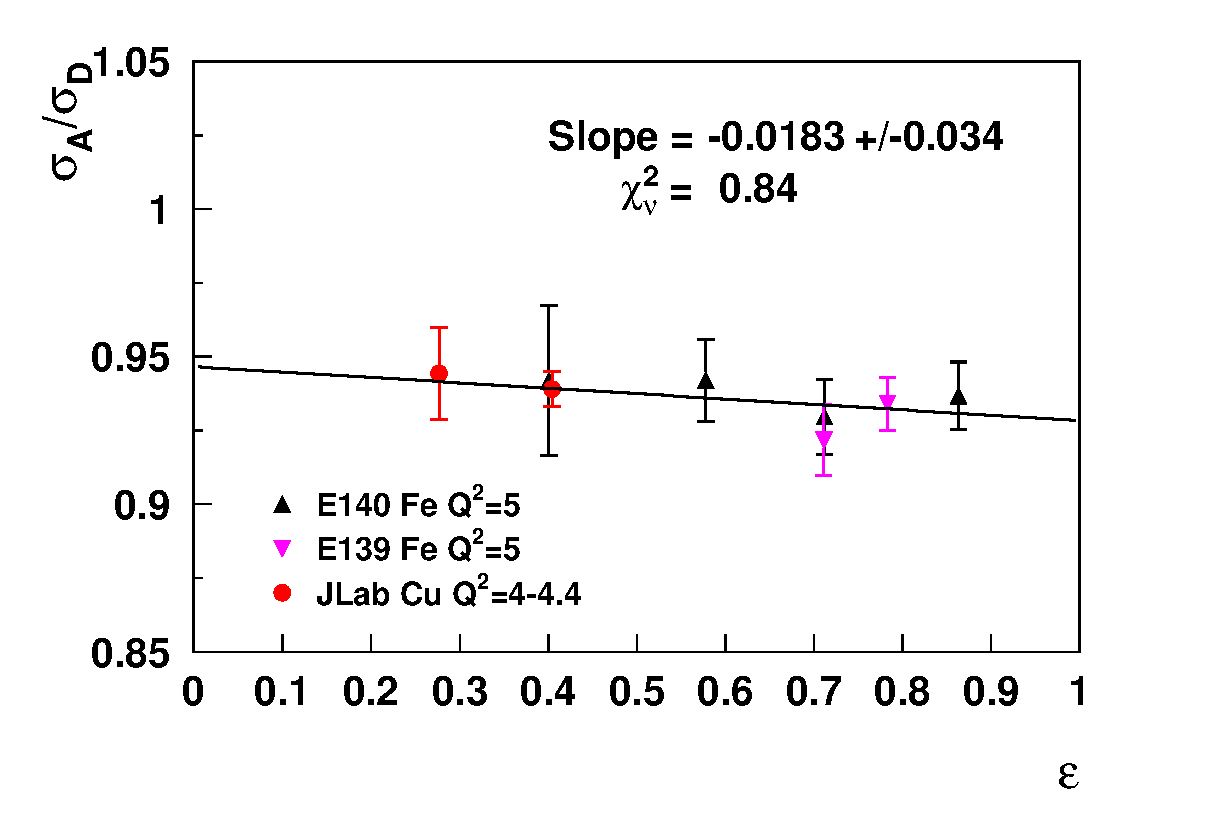
\includegraphics[width=.44\textwidth,height=55mm]{plots/x0p5_epsdep_3expfit_nocc.eps}
%\includegraphics[width=.44\textwidth,height=55mm]{plots/x0p5_epsdep_3expfit_cc.eps}
%\caption{Extracted cross ratios using the updated data from
%~\cite{slace140,slace139} and E03-103 experiment as a function of $\epsilon$
%for the Fe/Cu targets for $x=0.5$ and $Q^2$ values as mentioned in the legend.
%\textit{Include the figure, or just point to preprint and analysis in
%preparation???.  Also, the quoted chi-squared value looks way too large for
%the bottom plot; presumably this is the floating normalizations, but with 
%2 normalizations and 2 fit parameters, there are 4 degrees of freedom and
%it doesn't look like the total chi-squared could be 4 (looks more like 2).}
%\label{epsdep_cu_fig}}
%\end{center}
%\end{figure}
%
%
%
%Since the Coulomb correction factors are substantial for the heavy nuclei, it
%motivated us to investigate the details of this correction factors; in
%particular the impact of its strong angular dependence. The prescription used
%in the present analysis and the correction factors derived are discussed in
%detail in section~\ref{cc.ssec}. As mentioned in the introduction if $\epsilon
%=1$ or $R_{A_1} =R_{A_2}$ (the longitudinal to transverse virtual-photon
%absorption cross section for two different nuclei $A_1$ and $A_2$ ) then only
%one can identify the measured cross section ratios as the ratios of $F_2$
%structure functions (and hence as the EMC ratios) of the two different nuclei
%under investigation. This idea was tested in SLAC E140
%experiment~\cite{slace140}, which set limits on any possible nuclear
%dependence for $R$. They assumed the Coulomb distortion effects are small and
%did not include these corrections in their analysis. However, our re-analysis
%(by updating Coulomb corrections and including isoscalar corrections used in
%this analysis) of the SLAC 140~\cite{slace140}, SLAC E139~\cite{slace139} and
%an global analysis including preliminary results for the Cu target from E03-103
%data revealed a nontrivial nuclear dependence in
%$R_{A}-R_{D}$~\cite{Solvignon:2009it}.
%
%
%
%Figure~\ref{epsdep_cu_fig} shows the shows the $\epsilon$ dependence of
%extracted cross section ratios for the Cu (Fe target for SLAC experiments)
%target extracted for $x=0.5,$ $Q^2\sim 5$GeV$^2$ point. In this analysis,
%the data at low $\epsilon$ value from the E03-103 experiment are combined with
%the measurements from SLAC~\cite{slace140,slace139} to study the $\epsilon$
%dependence of the cross section ratios. The slope derived using a linear fit
%after taking care of the appropriate normalization uncertainties between 
%different experimental data sets is found to be consistent with zero (see top
%plot in figure~\ref{epsdep_cu_fig}). However, after the application of Coulomb
%corrections there is a non-trivial change in the slope (from -0.0183$\pm$0.034
%to -0.0602$\pm$0.0345) for the studied data set. If we assume there is no
%$\epsilon$ dependence for the cross section ratios, then the $\chi{^2}_{\nu}$
%values are 1.51 and 0.70 for the case with and with out Coulomb corrections
%applied, respectively. This analysis hints at the interesting fact that there
%may be a non-trivial $\epsilon$ dependence for the cross section ratios after
%the application of Coulomb corrections.
%
%\textit{Cite existing paper looking at this issue for low $Q^2$.  Mention that
%the nuclear dependence of R at high $x$ is under investigation and will be
%addressed in a forthcoming publication}
%
%
%\begin{figure}[htbp]
%\begin{center}
%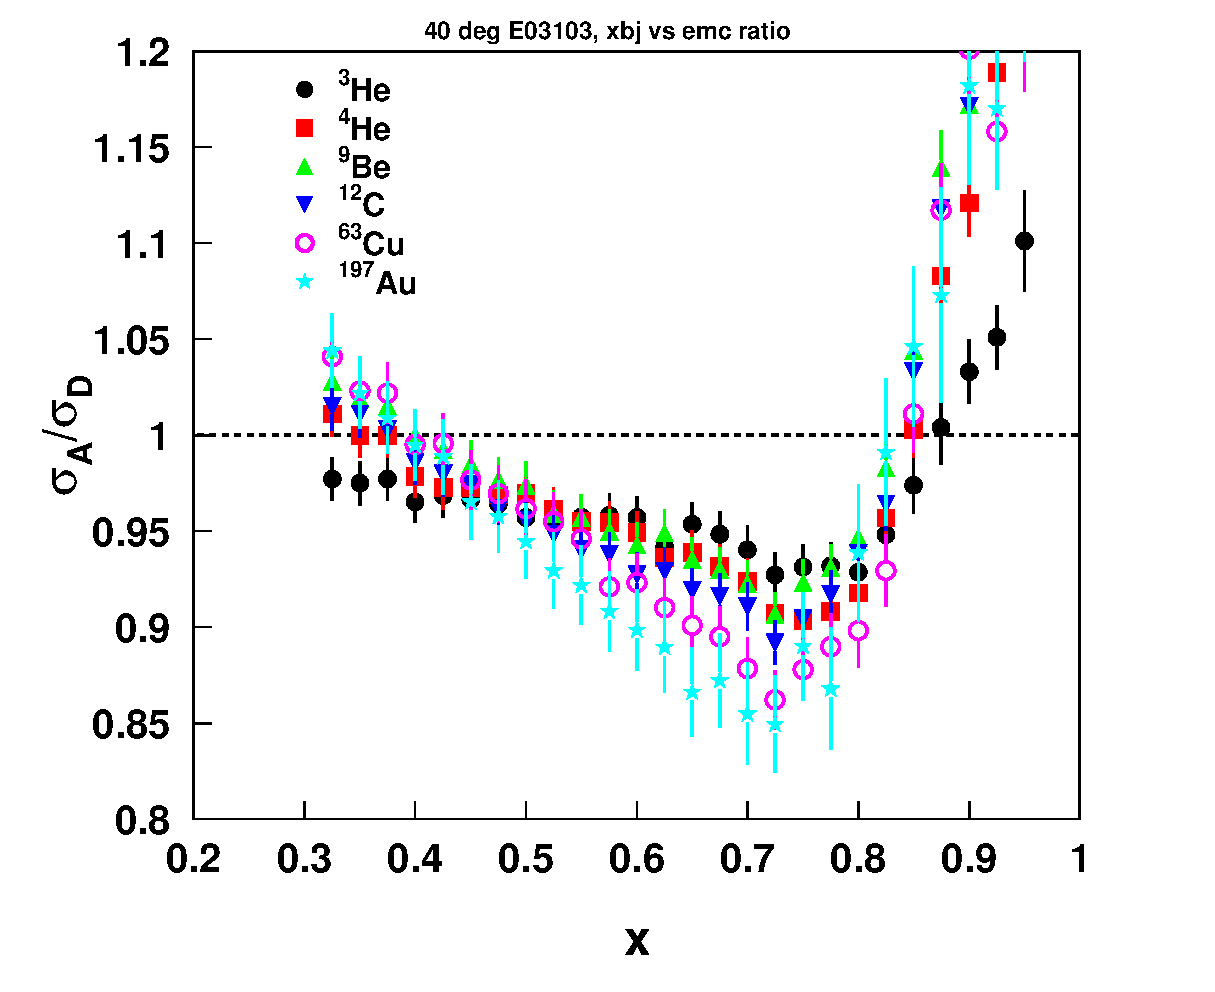
\includegraphics[width=.44\textwidth,height=55mm]{plots/e03103_40deg_emc_x_1zone.eps}
%\caption{EMC ratios for different targets as a function of $x$ for the 40
%degree data. \textit{JRA: Useful for us, but I don't think we want to show
%it, since we lead up to the issue based on the individual nuclei, and this
%is just a more cluttered version.  Only 'new' point it makes is that we see
%this same low-$x$ behavior in the context of our A dependence, rather than
%just in the us-vs-SLAC.}
%\label{emc_x_40deg_1zone_fig}}
%\end{center}
%\end{figure}
%
%The effects of binding and Fermi motion exist over the entire $x$ region, and
%not at just at the largest $x$ values. However, data at large $x$ allows for
%tests of the models chosen to describe binding and Fermi motion.
%Figure~\ref{emc_x_40deg_1zone_fig} shows the EMC ratios for different targets
%as a function of $x$ for the 40 degree data. \textit{More discussion about
%high x and low x cross overs??}.
%
%\textit{Potential impact: To the extent that it's normalization, it won't
%impact our EMC slopes, which is our primary evaluation of the overall size
%of the effect.  CSB (and RC?) disfavored, as would expect sharp rise at
%low $x$.}


%========================================================
\subsection{A dependence of the ratios}\label{adepresult.ssec}

%\textit{JRA: For now, removed figures showing EMC slope vs rho, A, A$^{-1/3}$,
%and separation energy - no real changes from trend in EMC/SRC paper. If we do
%want to show a couple a-dependence plots, include JLab and SLAC slopes
%separately, rather than showing the combined results.  Maybe a ln(A) scale,
%just for spacing not physics [and can compare to SLAC param. of EMC effect, to
%see how well it works].}

%\textit{JRA: Do we even need an A dependence section, or just talk about it
%global conclusions.  Probably worth 1-2 figures and some general discussion. 
%Should talk about $x_A$ vs $x_p$.  Do we have calculations for light nuclei?? 
%Do we compare to Kulagin and Petti (semi-mostly calculations)? Maybe this
%becomes an overall interpretation rather than A dependence section.}

%\begin{figure}[htbp]
%\begin{center}
%\includegraphics[angle=-90,width=.42\textwidth]{plots/emc_vs_dens_lp.eps}
%\includegraphics[angle=-90,width=.42\textwidth]{plots/emc_vs_dens_scaled_overlap_lp.eps}
%\includegraphics[angle=-90,width=.42\textwidth]{plots/emc_vs_a_lp.eps}
%\includegraphics[angle=-90,width=.42\textwidth]{plots/emc_vs_a_third_lp.eps}
%\includegraphics[angle=-90,width=.42\textwidth]{plots/emc_vs_ave_se_kulagin_lp.eps}
%\caption{EMC vs. stuff.}
%\label{emc_vs_stuff}
%\end{center}
%\end{figure}

%\textit{Maybe a discussion of the A dependence, from the data first (with
%plot(s) showing A, $\rho$ dependence.  We can then discuss fitting the
%A dependence, and just plug that into the parameterization discussion in
%the next section.}

Table~\ref{slope_emc_table} shows the EMC slopes extracted from data from
the SLAC experiment and this experiment. This table is an updated version of
table 1 provided in~\cite{arrington12c} which includes some of the updated
results from E03-103. These slopes are shown vs A in Fig.~\ref{XX}.
STATEMENT ON CONSISTENCY, IMPROVED PRECISION, NEW NUCLEI. Our light nuclei
results, in particular for $^9$Be, show a clear deviation from scaling with
density~\cite{seely09}, while the lightest nuclei show deviations from a
smooth scaling with $A$.  It has been suggested that the local density
or the overlap of the struck nucleon with nearby neighbors may drive the
scaling of the EMC effect~\cite{seely09, arrington12c,??}, or that off-shell
effects in the highly virtual nucleons may in fact be
responsible~\cite{weinstein11}.  In connection with these ideas, it has been
suggested that there may be both an A dependence and an isospin dependence,
with additional modification in neutron-rich nuclei~\cite{arrington12c,
hen13, sargsian12}.  This will be discussed in the following section.


%\textit{Actually, includes new heavy target data, modified (slightly) light
%target, AND updated SLAC data, right??}.


\begin{table}[htb]
\begin{center}
\caption{Combined EMC slopes, $|dR_{EMC}/dx|$, extracted from
SLAC~\cite{slace139,arrington12c} and this experiment.
\textit{JRA: THE SLAC NUMBERS ARE IDENTICAL TO THE EMC/SRC PAPER; SHOULDN'T
THEY HAVE THE UPDATED ISOSCALAR AND COULOMB CORRECTIONS?  SMALL BUT WORTH
INCLUDING SO THAT ALL OF OUR SLAC RESULTS ARE THE UPDATED VERSIONS.}}
\begin{tabular}{|c|c|c|c|}
\hline
A & JLAB E03-103& SLAC E139& Combined\\
\hline
$^3$He  & 0.087 $\pm$ 0.028 &        -          & 0.087 $\pm$ 0.028 \\
$^4$He  & 0.198 $\pm$ 0.027 & 0.191 $\pm$ 0.061 & 0.197 $\pm$ 0.025 \\
Be      & 0.267 $\pm$ 0.030 & 0.208 $\pm$ 0.038 & 0.245 $\pm$ 0.023 \\
C       & 0.280 $\pm$ 0.029 & 0.318 $\pm$ 0.041 & 0.292 $\pm$ 0.024 \\
Al      &        -          & 0.325 $\pm$ 0.034 & 0.325 $\pm$ 0.034 \\
$^{40}$Ca &       -         & 0.350 $\pm$ 0.047 & 0.350 $\pm$ 0.047 \\
Fe      &        -          & 0.388 $\pm$ 0.032 & 0.388 $\pm$ 0.032 \\
Cu      & 0.408 $\pm$ 0.037 &          -        & 0.408 $\pm$ 0.037 \\
Ag      &        -          & 0.496 $\pm$ 0.051 & 0.496 $\pm$ 0.051 \\
Au      & 0.484 $\pm$ 0.??? & 0.409 $\pm$ 0.039 & 0.436 $\pm$ 0.031 \\
\hline
\end{tabular}
\end{center}
\label{slope_emc_table}
\end{table}

\begin{figure}[htbp]
\begin{center}
\includegraphics[angle=-90,width=.42\textwidth]{plots/emc_slac_xem_vs_a_bars.eps}
\caption{EMC slope vs. A for SLAC E139 and JLab E03-103.}
\label{adep_slac_jlab}
\end{center}
\end{figure}


\subsection{Modified parametrization of the EMC effect}\label{emcparam.ssec}

\textit{UPDATED PARAMETERIZATION??  Want to make sure it doesn't have
pathologies at low/high x if we want to suggest it as an improvement.}

Though the parametrization of the EMC effect provided by SLAC
analysis~\cite{slace139} globally describes the presented data, it is
clear~\cite{seely09, arrington12c} that the EMC effect cannot be explained by a
simple ad-hoc logarithmic A-dependence or in terms of the average nuclear
density. Results from the light nuclei suggests that the nuclear modification
may depends on clustering effects and is mainly driven by the local
environment of the nuclei under examination. This motivated us to do a
detailed investigation of the modified parametrization for the EMC effect.

For the parametrization, we make use of the fact that the measurements show a
universal shape and a weak dependence on $A$. The data can be parameterized as
$\sigma{^A}/\sigma{^D}= 1.0 + f(x)~|dR^{A}_{EMC}/dx|$, where 
$\sigma{^A}/\sigma{^D}$ is the isoscalar corrected EMC ratios and
$|dR^{A}_{EMC}/dx|$ is the absolute value of the EMC slope for the
corresponding nuclei. As explained in ~\cite{seely09}, the magnitude of the
EMC effect is defined as the value of the slope of a linear fit,
$dR_{EMC}/dx$, to the cross section ratios for $0.35 < x < 0.7$. Here, f(x) is
polynomial fit done to the available world data for carbon to get the shape
($x$ dependence) of the EMC effect and is given by $f(x)= -0.28243 + 6.9324x
- 40.886x{^2} + 103.01x{^3} - 125.77x{^4} + 59.399x{^5}$. In this way a simple
connection can be made to the observed effect and the EMC slopes extracted for
the corresponding nuclei. These parametrization also describes the trends
observed in NMC~\cite{Amaudruz:1995tq,Arneodo:1995cs}, SLAC\cite{slace139}
data and are only valid in the region $0.01< x < 0.95$.


Though the resulting parametrization still depends on the mass number via the
slope and doesn't have the local properties or the details of the clustering
effects of the corresponding nuclei, it gives a better description of the
trends in the observed nuclear dependence. The A-dependent curves presented
here are plotted with extracted values of the combined EMC slopes as given in
Table~\ref{slope_emc_table}. However, for arbitrary nuclei, the EMC slopes
can be obtained from a linear fit to the mass dependence.
Figure~\ref{emcslopes_athird_fig} shows the A$^{-1/3}$ dependence of the
extracted slopes. Also shown is a linear fit (solid lines) for A$\geq$12.
The fit is limited up to A=12 and is based on the assumption that the nuclear
density distributions have a common shape and that for these medium-heavy
nuclei, the nuclear effects scale as a linear function of A$^{-1/3}$
\cite{sick_day_nucmatter,arrington12c}. However, as one can see from the
figure, the functional form 0.5530 - 0.6141~A$^{-1/3}$ gives a fairly
reasonable description of the magnitude of the EMC slopes observed even in the
light nuclei (dashed lines).

\begin{figure}[htbp]
\begin{center}
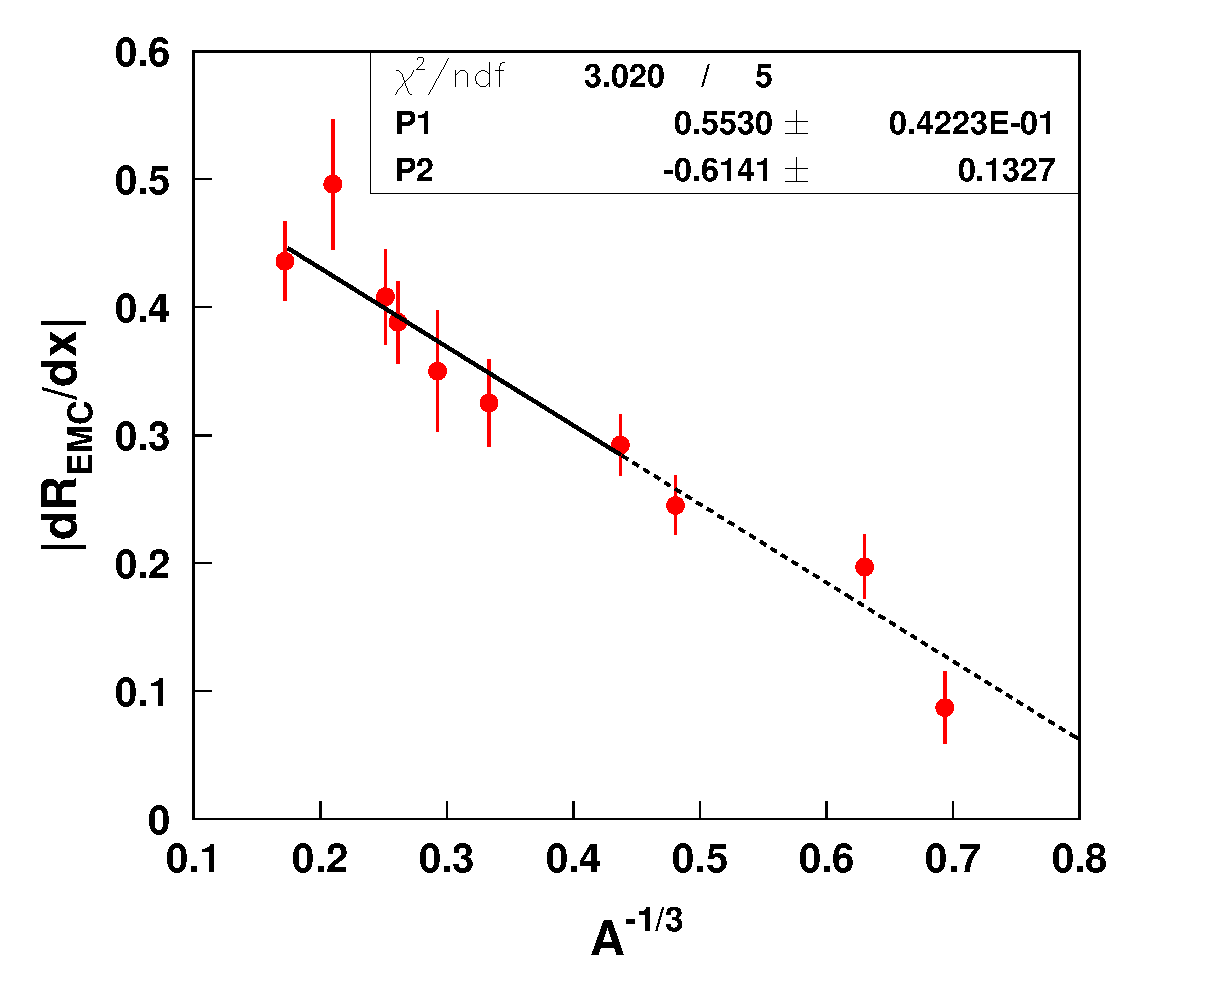
\includegraphics[width=.38\textwidth]{plots/emcslopes_athird.eps}
\caption{Magnitude of the extracted EMC slopes vs. A$^{-1/3}$. Here, the solid
lines shows the fit for nuclei with A$\geq$12, while the dashed line shows the
trend in A$^{-1/3}$ obtained from such a linear fit for the light
nuclei.\label{emcslopes_athird_fig}}
\end{center}
\end{figure}
%========================================================
\subsection{SRC-EMC discussion}

\begin{figure}[htbp]
\begin{center}
\includegraphics[angle=-90,width=.46\textwidth]{plots/plotfit_all_norescaling_nocm_rean_final_lp.eps}
%\includegraphics[angle=-90,width=.46\textwidth]{plots/plotfit_all_norescaling_no_cm_force0_rean_final_lp.eps}
\includegraphics[angle=-90,width=.46\textwidth]{plots/plotfit_all_norescaling_nocm_rean_deut_final_lp.eps}
\caption{EMC vs SRC stuff.  Need to update Niso/Ntot correction.}
\label{emc_vs_src}
\end{center}
\end{figure}

\begin{figure}[htbp]
\begin{center}
\includegraphics[angle=-90,width=.46\textwidth]{plots/plotfit_all_nzaam1_xaxis_xyerr_rean_final_lp.eps}
%\includegraphics[angle=-90,width=.46\textwidth]{plots/plotfit_all_nzaam1_xaxis_force0_xyerr_rean_final_lp.eps}
\includegraphics[angle=-90,width=.46\textwidth]{plots/plotfit_all_nzaam1_xaxis_xyerr_rean_deut_final_lp.eps}
\caption{EMC vs SRC stuff.  Need to update Niso/Ntot correction.}
\label{emc_vs_src2}
\end{center}
\end{figure}

\textit{updated SRC-EMC plot with E03-103 heavy nuclei.  Need plots with
updated Ntot/Niso for LD, need chisquared values for LD fits without the
CM motion uncertainty for comparison.  Ntot/Niso shifts heavier nuclei to
the right, improving linear correlation.  In both cases, still see some
residual excess in Fe, Cu, Au (but not very significant in LD case).}

While there have been many theoretical models put forth as explanations for
the EMC effect during the last 30 years, a recent experimental observation has
emerged as a tantalizing possibility.  A suggestive correlation has been
established between the "insert synonym for EMC effect" and $a_2$ or $R_{2N}$,
the quantities connected to the relative number of high momentum nuclei or
short-range correlations relative to the deuteron~\cite{weinstein11, hen13,
arrington12c}.  The two quantities are connected by a center-of-mass motion
correction that needs to be applied to the raw $a_2$ ratio, which comes from
$A/D$ high momentum tails to account for the fact that the deuteron-like pair
in the $A$ nucleus is free to move around in the field of the other nucleons.
There have been two explanations offered for the linear relationship seen
between the SRC results and the EMC results.  The first~\cite{weinstein11}
suggests that it's the virtuality that's responsible for the nuclear
dependence of both quantities and a simple linear fit between $dR_{EMC}/dx$
and $a_2$ tests that hypothesis.  The second idea~\cite{arrington12c} links
the size of the EMC effect directly to the number of high-density nucleon
configurations, as the early data suggested ~\cite{seely09}, specifically,
$NN$ pairs.  As was established at Jlab~\cite{subedi08} and
BNL~\cite{piasetzky06}, the short-range correlation pairs are
overwhelmingly $np$, so to make a connection to all NN pairs, we need to scale
$R_{2N}$ by $A(A-1)/2)/NZ$ before doing our linear test. Several different
variations of this test were performed and are described in detail in
Ref.~\cite{arrington12c}.  However, the data does not conclusively favor one
explanation over the other.  We repeat the comparisons here, with new results
on heavy nuclei for the EMC effect, as well as updated results for the light
nuclei.  The results are summarized in Table.~\ref{tab:fits_summary} and the
fit using a deuteron constraint is shown in Fig.~\ref{fig:src_emc_fit}.

The results have not changed very much from what was presented
in~\cite{arrington12c}, as far as the EMC effect for the deuteron (zero by
definition), or the IMC effect in the deuteron (deviation from the sum of
neutron and proton structure functions).  However, the "goodness" of the fits
did move - with $chi^2$ improving for all the LD scenarios and getting worse
for the HV scenarios.  The extreme was for the case of the constrained
deuteron fit (using a deuteron point with errors to account for correlations
between the other points), with $chi^2$ of 10 and 4 for the LD and HV
hypotheses, respectively.

However, on the whole, the situation remains largely unchanged - with the need
for more data as urgent as ever.

\begin{figure}[h!]
\includegraphics[angle=270,width=0.45\textwidth]{plots/plotfit_all_norescaling_no_cm_force0_rean_final_lp.eps}
\includegraphics[angle=270,width=0.45\textwidth]{plots/plotfit_all_nzaam1_xaxis_force0_xyerr_rean_final_lp.eps}
\caption{Tests of the high virtuality (HV) and local density (LD) hypotheses
for the relationship between the A/D structure function ratios and SRC ratios.
The black line indicates a 2-parameter fit with no constraints and the red
dotted line is a fit with a string deuteron constraint (intercept required to
be zero).}
\label{fig:src_emc_fit}
\end{figure}


\begin{table}
\begin{center}
\caption{}
\label{tab:fits_summary}
\begin{tabular}{| c | c | c | c |}
\hline
TEST & $\chi ^2/NDF$ & slope & intercept\\
\hline
HV-0 & 1.47 & 0.0893 & N/A\\
HV-2 & 1.44 & 0.0906 & -0.0044\\
HV-D & 1.26 & 0.1067 & -0.0582\\
LD-0 & 0.57 & 0.0520 & N/A\\
LD-2 & 0.64 & 0.0541 & -0.0124\\
LD-D & 0.57 & 0.0522 & 0.011\\
\hline
\end{tabular}
\end{center}
\end{table}

